\documentclass[a4paper]{article}

\usepackage{a4wide}
\usepackage{amsmath}
\usepackage{amssymb}
\usepackage{amsthm}
\usepackage{enumerate}
\usepackage{multicol}
\usepackage{tikz}
\usepackage[utf8]{inputenc}


\theoremstyle{definition}
\newtheorem{problem}{Příklad}
\newtheorem*{ukol}{Domácí úkol}


\begin{document}

\section*{NAIL062 V\&P Logika: 3. cvičení}


\textbf{Témata:} 
Počítání výroků až na ekvivalenci (Lindenbaum-Tarského algebra výroků). 2-SAT a implikační graf. Horn-SAT a jednotková propagace. Algoritmus DPLL. Kódování problémů do SAT.


\medskip\begin{problem}
    Nechť $|\mathbb{P}|=n$ a mějme výrok $\varphi\in\mathrm{VF}_{\mathbb{P}}$ takový, že $|M(\varphi)|=m$. Určete počet až na ekvivalenci:
    \begin{enumerate}[(a)]
    \item výroků $\psi$ takových, že $\varphi \models \psi$ nebo $\psi \models \varphi$,
    \item teorií nad $\mathbb{P}$, ve kterých platí $\varphi$,
    \item úplných teorií nad $\mathbb{P}$ ve kterých platí $\varphi$,
    \item teorií $T$ nad $\mathbb{P}$ takových, že $T \cup \{\varphi\}$ je bezesporná.
    \end{enumerate}
    Uvažme navíc spornou teorii $\{\varphi,\psi\}$ kde $|M(\psi)|=p$. Spočtěte až na ekvivalenci:
    \begin{enumerate}[(a)]
    \item[(e)] výroky $\chi$ takové, že $\varphi \vee \psi \models \chi$, 
    \item[(f)] teorie, ve kterých platí $\varphi \vee \psi$.
    \end{enumerate}
\end{problem}

    
\medskip\begin{problem} Sestrojte implikační graf daného 2-CNF výroku. Je splnitelný? Pokud ano, najděte nějaké řešení.
\begin{enumerate}[(a)]
    \item $(p_1\vee \neg p_2)\wedge (p_2\vee p_3)\wedge (\neg p_3\vee \neg p_1)\wedge (\neg p_3\vee \neg p_4)\wedge (p_4\vee p_5)\wedge (\neg p_5\vee \neg p_1)$,
    \item $(p_1\vee \neg p_2)\wedge (p_2\vee p_3)\wedge (\neg p_3\vee p_1)\wedge (\neg p_3\vee \neg p_4)\wedge (p_4\vee p_5)\wedge (\neg p_5\vee p_1)$,
    \item $(p_0 \vee  p_2) \wedge  (p_0 \vee  \neg p_3) \wedge  (p_1 \vee  \neg p_3) 
    \wedge  (p_1 \vee  \neg p_4) \wedge  (p_2 \vee  \neg p_4) 
    \wedge  (p_0 \vee  \neg p_5)
    \wedge 
    (p_1 \vee  \neg p_5) \wedge  (p_2 \vee  \neg p_5) \wedge  (\neg p_1 \vee  \neg p_6) \wedge  (p_4 \vee  p_6) \wedge  (p_5 \vee  p_6) \wedge  p_1\wedge \neg p_7$.
\end{enumerate}
\end{problem}


\medskip\begin{problem}
Pomocí jednotkové propagace zjistěte, zda je následující Hornův výrok splnitelný. Pokud ano, najděte nějaké splňující ohodnocení.
\begin{align*}
    &(\neg p_1 \vee \neg p_3 \vee p_2)\wedge(\neg p_1 \vee p_2)\wedge p_1 \wedge (\neg p_1 \vee \neg p_2 \vee p_3)\wedge \\
    &(\neg p_2 \vee \neg p_4 \vee p_1)\wedge(\neg p_4 \vee \neg p_3 \vee \neg p_2)\wedge(p_4\vee \neg p_5 \vee\neg p_6)
\end{align*}
\end{problem}
    

\medskip\begin{problem}
    Pomocí algoritmu DPLL rozhodněte, zda je následující CNF formule splnitelná.
    \begin{enumerate}[(a)]
        \item $$ (\neg p_1 \wedge \neg p_2)\land( \neg p_1 \wedge p_2)\land( p_1 \wedge \neg p_2)\land( p_2 \wedge \neg p_3)\land( p_1 \wedge p_3)$$
        \item \begin{align*}
            &(\neg p_1 \wedge p_3 \wedge p_4)\vee( \neg p_2 \wedge p_6 \wedge p_4)\vee( \neg p_2 \wedge \neg p_6 \wedge \neg p_3)\vee(
                \neg p_4 \wedge \neg p_2)\vee \\ & ( p_2 \wedge \neg p_3 \wedge \neg p_1)\vee ( p_2 \wedge p_6 \wedge p_3)\vee
                ( p_2 \wedge \neg p_6 \wedge \neg p_4)\vee
                ( p_1 \wedge p_5)\vee \\ & ( p_1 \wedge p_6)\vee(
                \neg p_6 \wedge p_3 \wedge \neg p_5)\vee( p_1 \wedge \neg p_3 \wedge \neg p_5)    
        \end{align*}
    \end{enumerate}
\end{problem}


\medskip\begin{problem}
Lze šachovnici $4\times 4$ bez dvou protilehlých rohů perfektně pokrýt kostkami domina? Zakódujte tento problém do SAT. Zobecněte na všechna sudá~$n$.
\end{problem}
    
    
\medskip\begin{problem}
    Lze obarvit čísla od 1 do $n$ dvěma barvami tak, že neexistuje monochromatické řešení rovnice
    $a+b=c$ s $1\leq a<b<c\leq n$? Sestrojte výrokovou formuli $\varphi_n$ v CNF která je splnitelná, právě když to lze. Zkuste nejprve $n=8$.
    
    Zkuste si doma: Napište skript generující $\varphi_n$ v DIMACS CNF formátu. Použijte SAT solver k nalezení nejmenšího $n$ pro které takové obarvení neexistuje (tj. každé 2-obarvení obsahuje monochromatickou trojici $a<b<c$ takovou, že $a+b=c$).
\end{problem}

    
\medskip\begin{problem}
    Zakódujte problém setřídění trojice celých čísel do SAT.
\end{problem}
    
        
\medskip\begin{problem}
Věta o čtyřech barvách říká, že následující mapy lze obarvit 4 barvami tak, že žádné dva sousedící regiony nemají stejnou barvu. Najděte takové obarvení pomocí SAT solveru.
\begin{multicols}{2}
\begin{enumerate}[(a)]
    \item Mapa krajů Česka  
    
    \vfill 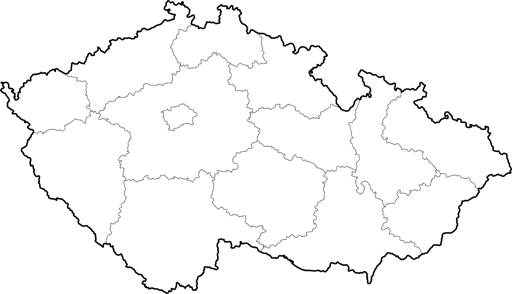
\includegraphics[width=0.45\textwidth]{files/map-coloring-czechia.png} \vfill
    
    \item Těžší instance  
    
    \vfill 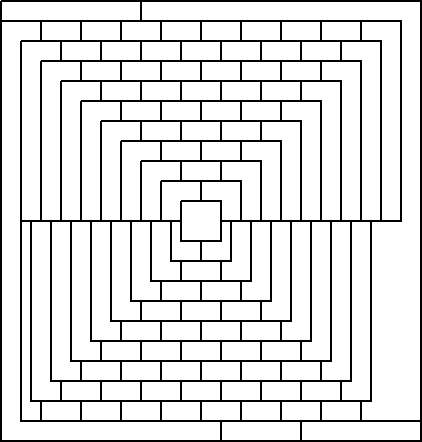
\includegraphics[width=0.45\textwidth]{files/map-coloring-hard.png} \vfill
\end{enumerate}
\end{multicols}
\end{problem}



\medskip\begin{ukol}[3 body]
\begin{enumerate}[1.]
\item Pomocí algoritmu implikačního grafu najděte všechny modely následující teorie:
$$
T=\{p,\neg q \to \neg r,\neg q \to \neg s,r \to p,\neg s \to \neg p\}
$$

\item Pomocí algoritmu jednotkové propagace najděte všechny modely následující teorie:
\begin{align*}
    &(\neg a \vee \neg b \vee c \vee \neg d)\wedge(\neg b \vee c)\wedge d \wedge (\neg a \vee \neg c \vee e)\wedge \\
    &(\neg c \vee \neg d)\wedge(\neg a \vee \neg d \vee \neg e)\wedge(a\vee \neg b \vee\neg e)
\end{align*}

\item Uvažme následující výroky $\varphi$ a $\psi$ nad $\mathbb P=\{p, q, r, s\}$:
\begin{align*}
    \varphi &= (\neg p \vee  q)\to(p\wedge r)\\
    \psi &= s\to q
\end{align*}
\begin{enumerate}[(a)]
    \item Určete počet (až na ekvivalenci) výroků $\chi$ nad $\mathbb P$ takových, že $\varphi\wedge\psi\models\chi$.
    \item Určete počet (až na ekvivalenci) úplných teorií $T$ nad $\mathbb P$ takových, že $T\models\varphi\wedge\psi$.
    \item Najděte nějakou axiomatizaci pro každou (až na ekvivalenci) úplnou teorii $T$ nad $\mathbb P$ takovou, že $T\models\varphi\wedge\psi$.
\end{enumerate}
\end{enumerate} 
\end{ukol}

\end{document}